\documentclass[aps,prl,twocolumn,superscriptaddress,amsmath,amssymb,reprint]{revtex4-2}
\usepackage{graphicx}
\usepackage{bm}
\usepackage[colorlinks,allcolors=blue]{hyperref}
\newcommand{\Lc}{\mathcal{L}}
\newcommand{\Cc}{\mathcal{C}}

\begin{document}

\title{Chiral switching of many-body steady states is a cusp--hysteresis effect\\ with an exponentially long, but finite, lifetime}

\author{[Author list to be completed]}
\date{\today}

\begin{abstract}
Slowly driving a dissipative Rydberg gas around a closed loop in parameter space switches it between two collective steady states, and the switching depends on the direction of travel. The effect was recently observed and attributed to a mean-field ``Liouvillian exceptional structure'': two exceptional lines (ELs) of coalescing steady states that merge at a third-order exceptional point (EP3). We revisit this effect with the exact, permutation-symmetric Liouvillian of $N$ atoms and establish three results. (i) At mean-field level the ELs are saddle-node fold lines and the EP3 is the cusp. The final state is fixed by which fold the trajectory last crossed, so encircling the EP3 is neither necessary nor sufficient for switching. (ii) For every finite $N$ the steady state is unique and nondegenerate. Mean-field bistability reappears as a real Liouvillian eigenvalue $\lambda_{\rm sw}\propto e^{-sN}$. The finite-$N$ remnant of each EL is a genuine Liouvillian EP between the switching mode and the intrabasin relaxation mode. It lies at complex detuning and approaches the real axis as $e^{-0.156N}$. (iii) The chirality $\Cc$ obeys the scaling law $\Cc=F(T\lambda_{\min}(N))$, where $T$ is the loop period. Switching is therefore robust only inside the window $\gamma^{-1}\ll T\ll\lambda_{\min}^{-1}\sim e^{sN}$, and it is erased beyond it. For mesoscopic ensembles ($N\sim 20$--$40$) this erasure falls within experimental reach.
\end{abstract}

\maketitle

\emph{Introduction.}---Encircling an exceptional point (EP) of a non-Hermitian generator produces chiral state transfer. Its outcome depends on the direction of encirclement, not on the starting state~\cite{Doppler2016,SunYi2024}. Chiral transfer near Liouvillian EPs has been observed in single-qubit and single-photon settings~\cite{Gao2025}. In those settings it is a transient phenomenon, because the EP lives among decaying eigenmodes. Xie \textit{et al.}~\cite{Xie2025} reported a striking many-body version in a thermal Rydberg vapor~\cite{Carr2013}. Driving the coupling detuning and probe Rabi frequency around a loop switches the gas between its high- and low-transmission steady states in only one sense of rotation. Within a mean-field (MF) Lindblad description, the boundaries of the bistable region were identified as second-order Liouvillian ELs of coalescing \emph{steady states}, terminating at an EP3~\cite{Xie2025,SunYi2024}. Because all coalescing states have zero eigenvalue, the effect was argued to persist at long times. It was also argued to be distinct from simple hysteresis. Ref.~\cite{Xie2025} additionally formulated an empirical sufficient condition for switching: the two intersections of the trajectory with the ELs nearest to the initial point must lie on opposite sides of the EP3.

This interpretation raises a sharp question. The MF Liouvillian is nonlinear, while the true $N$-body Liouvillian $\Lc_N$ is linear. For finite $N$, $\Lc_N$ generically has a unique steady state. Moreover, a zero eigenvalue cannot be defective~\cite{HuBudich2025}. What, then, is the exact many-body counterpart of the steady-state EL and EP3? How long does the chiral switching survive? We answer both questions for the standard minimal model of a dissipative Rydberg ensemble, using the exact permutation-symmetric Liouvillian up to $N=60$.

\emph{Model.}---We consider $N$ two-level atoms ($|g\rangle$, Rydberg state $|e\rangle$) with uniform all-to-all interactions $V/N$. This is the setting in which MF theory becomes exact as $N\to\infty$:
\begin{equation}
\hat H=-\Delta\hat N_e+\Omega\hat J_x+\frac{V}{2N}\hat N_e(\hat N_e-1),\quad
\dot\rho=\Lc_N\rho,
\label{eq:H}
\end{equation}
with local decay $\hat L_i=\sqrt{\gamma}\,\hat\sigma_i^-$ and $\gamma\equiv1$. Here $\hat N_e=\sum_i|e\rangle_i\langle e|$ and $\hat J_x=\frac12\sum_i\hat\sigma_i^x$. $\Lc_N$ is permutation invariant, so it acts on a space of dimension $\binom{N+3}{3}$~\cite{Shammah2018}. This is $39\,711$ for $N=60$, which allows sparse shift-invert diagonalization and implicit (BDF2) time evolution. As a check, we reproduced the brute-force steady state for $N=3$ to $10^{-8}$. At MF level, Eq.~\eqref{eq:H} gives single-atom Bloch equations with the effective detuning $\tilde\Delta=\Delta-Vn$, where $n=\langle\hat N_e\rangle/N$. This is the same nonlinearity used in Ref.~\cite{Xie2025}. We take $V=10$ throughout.

\emph{Mean-field picture: folds and cusp.}---The stationary MF populations solve the cubic
\begin{equation}
n\big[(\Delta-Vn)^2+\tfrac14+\tfrac{\Omega^2}{2}\big]=\tfrac{\Omega^2}{4}.
\label{eq:cubic}
\end{equation}
Three real roots exist inside a wedge-shaped region [Fig.~\ref{fig:mf}(a)]. Two of them are stable and one is a saddle. The wedge boundaries are the lines where the cubic has a double root, i.e., saddle-node \emph{fold} bifurcations. A triple root occurs at the two \emph{cusp} points, $2V^2n_0^3-\frac34V^2n_0^2+\frac14=0$, $\Delta_c=\frac32Vn_0$, $\Omega_c=2Vn_0^{3/2}$. For $V=10$ these give $(\Delta_c,\Omega_c)=(5.485,4.422)$ and $(0.950,0.319)$. In the language of Refs.~\cite{Xie2025,SunYi2024}, the folds are the ELs and the cusps are EP3's. However, the Jacobian at a fold has one simple zero eigenvalue and remains diagonalizable. The coalescence is between \emph{fixed points of a nonlinear flow}, not between eigenvectors of a linear generator.

This identification immediately settles which loops switch. Inside the wedge, a slowly driven state follows the stable branch it is on. Leaving the wedge across a fold destroys one branch and forces a jump to the other. Entering the wedge across the left (right) fold places the system on the high-$n$ (low-$n$) branch, the only one that existed outside. Consider the start point $P_0$ and the maximal bistable arc of the loop that contains it. \emph{The final state depends only on which fold bounds that arc on the side the trajectory enters from.} It is therefore independent of the initial branch, and $\Cc=\pm1$ exactly when the two ends of the arc lie on different folds. Encircling a cusp is \emph{sufficient} if the loop crosses the wedge only once. It is not \emph{necessary}: loop B in Fig.~\ref{fig:mf}(a) never encloses a cusp, yet it re-enters the wedge through the opposite fold and switches as cleanly as loop A [Fig.~\ref{fig:mf}(b)]. Conversely, a loop whose bistable arc is entered and left through the same fold does not switch: a circle through $P_0$ that crosses only the left fold returns to the high branch for both senses and both initial branches ($n=0.399$ at $T=10^3$). This fold rule is the dynamical content of the empirical condition of Ref.~\cite{Xie2025}: here it is derived, shown to be also necessary, and seen not to require encirclement. The MF chirality is thus a hysteresis property of the fold geometry. ``Direction-dependent final state'' and ``chirality reverses with initial state'', both observed in Ref.~\cite{Xie2025}, are two descriptions of the same initial-state-independent outcome.

\begin{figure}[t]
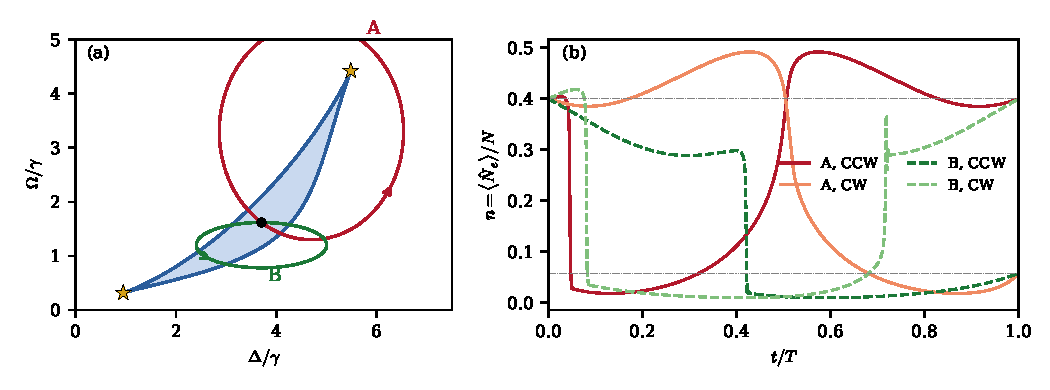
\includegraphics[width=\columnwidth]{../figs/fig1.pdf}
\caption{Mean-field geometry. (a)~Bistable wedge (shaded) bounded by fold lines (blue), which are the ``exceptional lines'' of Ref.~\cite{Xie2025}, meeting at two cusps (stars, ``EP3''). Loop A encloses the upper cusp; loop B encloses neither cusp. Both start at $P_0=(3.704,1.619)$ (dot). (b)~MF population along the loops ($T=10^3$), starting on the high branch. Both loops are chiral. Starting on the low branch (not shown) gives identical final states.}
\label{fig:mf}
\end{figure}

We also integrated the MF ladder models of Ref.~\cite{Xie2025} with their published fit parameters. In the three-level model (no microwave), the experimental $(\Omega_p,\Delta_c)$ loop gives a final state that is independent of the initial branch and fixed by the direction: $n=0.059$ (CW) and $0.198$ (CCW) at $T=50$. The cusp of this model sits at $(\Omega_p,\Delta_c)/2\pi\simeq(7.45,-30.1)$\,MHz, \emph{outside} the loop ($\Omega_p/2\pi\geq8.79$\,MHz). This conclusion is not robust to the fit, however. Changing any single fit parameter by $\pm10$--$20\%$ moves the cusp to $\Omega_p/2\pi$ between $6.4$ and $9.1$\,MHz, or pushes the low-$\Omega_p$ end of the wedge above $8$\,MHz. We therefore read this as an illustration, not as proof that the experiment did not encircle the EP3.

The four-level microwave-dressed model is more decisive. It reproduces the measured phase diagram of Ref.~\cite{Xie2025}, Fig.~1(f) (wedge from $\Delta_c/2\pi\simeq-57$\,MHz at small $\Omega_{\rm mw}$ to the cusp at $(\Delta_c,\Omega_{\rm mw})/2\pi\simeq(-73,70)$\,MHz), once the detuning modulation of the loops is taken as $\Delta_c=\Delta_0+\delta\sin\theta$. This sign makes the loops coincide with those drawn in that figure; the sign printed in their Methods does not. With it, the quasi-static MF outcomes of all three published loops agree with the measurements (their Fig.~3 and S3): the black and magenta loops switch and the cyan loop does not. Only the magenta loop encloses the cusp. The black loop never reaches it ($\Omega_{\rm mw}/2\pi\leq53$\,MHz), yet it switches because it crosses both folds. The cyan loop is the same ellipse with its $\Delta_c$ excursion removed on one half, so it leaves and re-enters through the same fold and does not switch. This is a direct experimental instance of the fold rule: switching without encircling, and no switching when one fold is crossed twice.

\emph{Exact Liouvillian: no degeneracy, exponential metastability.}---For finite $N$ the spectrum of $\Lc_N$ changes qualitatively [Fig.~\ref{fig:spec}(a)]. The zero eigenvalue is simple everywhere, including deep inside the wedge. Bistability manifests as a single isolated real eigenvalue $\lambda_1=-\lambda_{\rm sw}$, separated by an $O(1)$ gap from the rest of the spectrum. This is the standard spectral signature of first-order dissipative transitions~\cite{Minganti2018,Casteels2017,Macieszczak2016}. Inside the wedge $\lambda_{\rm sw}$ decays exponentially, $\lambda_{\rm sw}\propto e^{-s(\Delta,\Omega)N}$ [Fig.~\ref{fig:spec}(b)]. The barrier $s$ vanishes at the folds and is maximal near the coexistence line; at $\Omega=2$ we find $s_{\max}=0.117$ at $\Delta\simeq4.0$. In this regime the dynamics restricted to times $t\gg1$ is that of a classical two-state system. Its metastable states $\rho_{\rm hi},\rho_{\rm lo}$ are the extreme points of $\rho_{\rm ss}+c\,r_1$, where $r_1$ is the right eigenvector of $\lambda_1$~\cite{Macieszczak2016}. Writing $\rho(t)\simeq p\,\rho_{\rm hi}+(1-p)\rho_{\rm lo}$ gives
\begin{equation}
\dot p=-\lambda_{\rm sw}(\bm\theta(t))\,[\,p-p_{\rm ss}(\bm\theta(t))\,],
\label{eq:twostate}
\end{equation}
where $\bm\theta=(\Delta,\Omega)$ and $p_{\rm ss}$ is the weight of $\rho_{\rm hi}$ in $\rho_{\rm ss}$. Equation~\eqref{eq:twostate} is the exact large-$N$ content of the MF ``steady-state landscape''. At a fixed point inside the wedge both $p$ and $1-p$ are allowed only for $t\ll\lambda_{\rm sw}^{-1}$. In this regime, recent large-deviation analyses identify $1/N$ as an effective temperature in an Arrhenius law~\cite{Xiang2026}.

\emph{What replaces the EL.}---We find that the MF fold line has a precise finite-$N$ remnant. It is an ordinary Liouvillian EP, but not among zero modes. Approaching the left fold from outside, the two slowest decay modes undergo an avoided crossing near $\lambda\approx-0.76$ [inset region of Fig.~\ref{fig:spec}(a)]. These are the switching mode, which becomes intra-wedge metastability, and the intrabasin relaxation mode of the high branch, whose MF counterpart is the real Jacobian eigenvalue $\simeq-0.75$ of the high branch. Continuing $\Delta$ into the complex plane, we locate an exact EP2 of $\Lc_N$ at $\Delta_{\rm EP}(N)$. There $\lambda_1$ and $\lambda_2$ and their eigenvectors coalesce, with residual discriminant $<10^{-12}$ and eigenvector overlap $1-2\times10^{-14}$ at $N=30$. Figure~\ref{fig:spec}(c) shows that ${\rm Im}\,\Delta_{\rm EP}\propto e^{-0.156N}$ for $N\geq30$. Meanwhile ${\rm Re}\,\Delta_{\rm EP}$ drifts monotonically toward the fold; empirical fits $a+bN^{-p}$ with $p\in[1/2,1]$ extrapolate to $3.43$--$3.63$, bracketing the MF fold at $3.60$. In the thermodynamic limit, an exponentially pinched EP between the two slowest \emph{decaying} modes thus reaches the real axis at the fold. There the switching rate turns into a relaxation rate and the metastable branch ends. The ``steady-state EL'' is the limit of this object rather than a degeneracy of steady states. This is consistent with the no-go theorem of Ref.~\cite{HuBudich2025}.

\begin{figure*}[t]
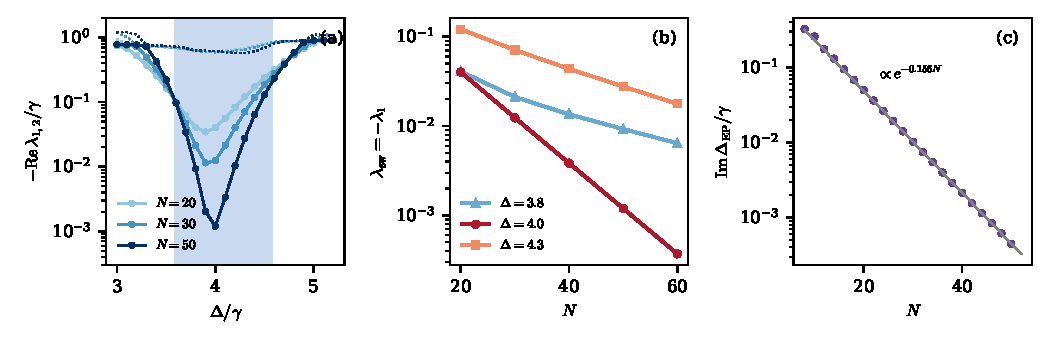
\includegraphics[width=\textwidth]{../figs/fig2.pdf}
\caption{Exact spectrum of $\Lc_N$. (a)~Slowest decay rates $-{\rm Re}\,\lambda_1$ (lines with dots) and $-{\rm Re}\,\lambda_2$ (dotted) versus $\Delta$ at $\Omega=2$, for $N=20,30,50$. The MF wedge is shaded. The zero mode (not shown) is always simple. (b)~Exponential closing of the switching rate inside the wedge. (c)~Imaginary part of the detuning of the exact EP2 between $\lambda_1$ and $\lambda_2$ that is associated with the left fold. The line is an exponential fit to $N\geq30$.}
\label{fig:spec}
\end{figure*}

\emph{Chirality window and its erasure.}---We now drive loops A and B with period $T$, starting from $\rho_{\rm hi}$ at $P_0$, and define the chirality
\begin{equation}
\Cc(T,N)=\frac{n_{\rm CCW}(T)-n_{\rm CW}(T)}{n_{\rm hi}(P_0)-n_{\rm lo}(P_0)},
\end{equation}
where $n_{\rm CCW/CW}$ are the populations after one counterclockwise/clockwise period. Thus $\Cc=\pm1$ means perfect switching and $\Cc=0$ means no memory of the direction. Figure~\ref{fig:chi}(a) compares exact BDF2 evolution of $\Lc_N$ ($N=10,20,30$; symbols) with Eq.~\eqref{eq:twostate} (lines). The reduction captures the full crossover; it overestimates $|\Cc|$ by $\lesssim15\%$, mostly from non-adiabatic losses at short $T$. Starting from $\rho_{\rm lo}$ or $\rho_{\rm ss}$ gives identical final states (checked for $N=10$), so $\Cc$ is a property of the loop alone.

Three regimes appear. For $T\lesssim10$ the drive is non-adiabatic within each basin, so neither picture applies. For $10\ll T\ll\lambda_{\rm min}^{-1}$, $|\Cc|\to1$ as $N$ grows ($|\Cc|=0.62,0.95,0.995,0.999$ for $N=10,20,30,40$ on loop A). Here $\lambda_{\min}$ is the smallest switching rate on the arc through which the system must keep its memory. In this regime both loops A and B are chiral, with the sign fixed by the fold rule. For $T\gg\lambda_{\rm min}^{-1}$ the state follows $\rho_{\rm ss}(\bm\theta)$, which is a single-valued function of the parameters, and chirality is erased: $\Cc\to0$ for \emph{any} loop. Integrating Eq.~\eqref{eq:twostate} along the arc gives $|\Cc|\simeq\exp[-\oint\lambda_{\rm sw}\,dt]$ for the population that must stay metastable. This implies the one-parameter scaling $\Cc=F_{\rm loop}(T\lambda_{\min}(N))$, which Fig.~\ref{fig:chi}(b) confirms. The erasure time $T_{1/2}$, defined by $|\Cc|=1/2$, satisfies $T_{1/2}\lambda_{\min}\to43$ (A) and $19$ (B). It grows as $T_{1/2}=1.1\times10^3,4.1\times10^3,1.3\times10^4$ for $N=20,30,40$, i.e., $\propto e^{sN}$ with $s\approx0.12$.

\begin{figure}[t]
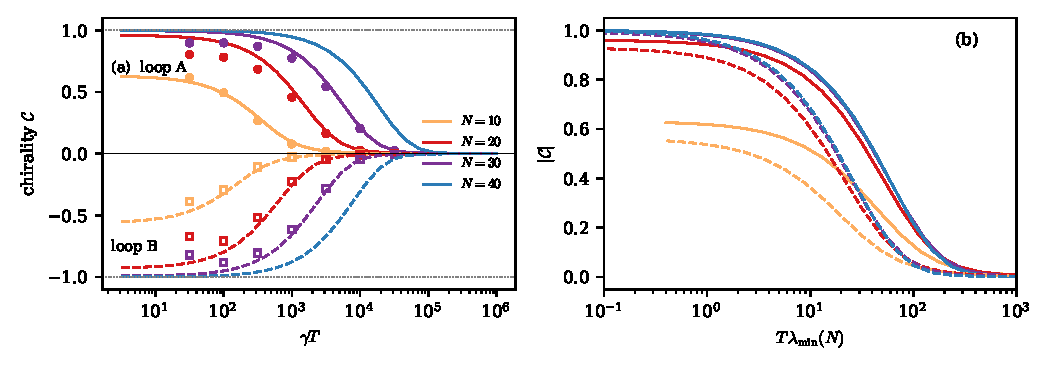
\includegraphics[width=\columnwidth]{../figs/fig3.pdf}
\caption{(a)~Chirality versus loop period for loops A ($\Cc>0$, solid) and B ($\Cc<0$, dashed). Symbols: exact evolution of $\Lc_N$. Lines: two-state reduction, Eq.~\eqref{eq:twostate}. (b)~Collapse of $|\Cc|$ onto a single curve per loop when $T$ is rescaled by the minimal switching rate $\lambda_{\min}(N)$ on the switching arc. Curves for $N=30$ and $40$ coincide.}
\label{fig:chi}
\end{figure}

\emph{Discussion.}---Our results recast many-body chiral switching in terms that are both less exotic and more predictive. The MF fold rule sharpens a condition already identified empirically in Ref.~\cite{Xie2025}; the new content is the exact finite-$N$ structure and the resulting chirality window. The robust ingredients are (a)~a fold geometry with a cusp, which fixes the sign of $\Cc$ by a hysteresis rule, and (b)~a metastable two-state manifold whose lifetime $\lambda_{\rm sw}^{-1}\sim e^{sN}$ sets the upper edge of a finite adiabatic window. The ``exceptional'' content of the problem is real but resides elsewhere. It is a genuine EP2 of the linear $N$-body Liouvillian between the switching and intrabasin relaxation modes, pinched onto the real axis as $e^{-0.156N}$. This mirrors the general mechanism of asymptotic exceptional steady states~\cite{HuBudich2025}. Single-particle chiral transfer near Liouvillian EPs is likewise lost at long times~\cite{Gao2025}. The difference here is that the loss time is exponentially long in $N$, which is why the effect looks stationary in a macroscopic vapor.

These statements are experimentally testable. In a thermal vapor ($N\to\infty$ effectively) one is always deep inside the window, consistent with Ref.~\cite{Xie2025}. Two signatures distinguish the present picture from EP encirclement. First, a non-encircling loop also switches, with the sign given by the fold rule; the black microwave loop of Ref.~\cite{Xie2025} already realizes this. Second, a cusp-enclosing loop that re-enters the wedge through the same fold does not switch. In mesoscopic ensembles, such as blockaded clouds, optical-tweezer arrays, or atoms in a cavity with all-to-all coupling, $N\sim20$--$40$ gives $T_{1/2}\sim10^3$--$10^4\,\gamma^{-1}$. For Rydberg decay rates $\gamma/2\pi\sim10$~kHz this is $T_{1/2}\sim$~ms. The predicted erasure of chirality and the data collapse $\Cc=F(T\lambda_{\min})$ should then be directly observable, with $\lambda_{\min}$ measured independently from the decay of transmission telegraph noise. More generally, any claim of ``exceptional'' steady-state physics derived from a nonlinear MF generator should be checked against the timescale $\lambda_{\rm sw}^{-1}$ of the linear many-body Liouvillian. Outside $\gamma^{-1}\ll T\ll\lambda_{\rm sw}^{-1}$ the effect does not exist.

\emph{Limitations.}---We used the minimal two-level model with uniform all-to-all interactions. For the ladder models of Ref.~\cite{Xie2025} we checked only the MF fold rule, not the finite-$N$ spectrum. Short-range interactions and Doppler broadening in vapors modify $s(\bm\theta)$, not the topology of the fold rule. The $N\to\infty$ location of the exact EP is extrapolated from $N\leq50$.

\emph{Data availability.}---All code and data underlying the figures are provided with this manuscript.

\begin{thebibliography}{99}
\bibitem{Doppler2016} J.~Doppler \textit{et al.}, Dynamically encircling an exceptional point for asymmetric mode switching, Nature \textbf{537}, 76 (2016).
\bibitem{SunYi2024} K.~Sun and W.~Yi, Encircling the Liouvillian exceptional points: a brief review, AAPPS Bull. \textbf{34}, 22 (2024).
\bibitem{Gao2025} H.~Gao, K.~Sun, D.~Qu, K.~Wang, L.~Xiao, W.~Yi, and P.~Xue, Photonic chiral state transfer near the Liouvillian exceptional point, Phys. Rev. Lett. \textbf{134}, 146602 (2025).
\bibitem{Xie2025} C.~Xie, K.~Sun, K.-D.~Wu, C.-F.~Li, G.-C.~Guo, W.~Yi, and G.-Y.~Xiang, Chiral switching of many-body steady states in a dissipative Rydberg gas, Sci. Bull. \textbf{70}, 3345 (2025); arXiv:2402.02779.
\bibitem{Carr2013} C.~Carr, R.~Ritter, C.~G.~Wade, C.~S.~Adams, and K.~J.~Weatherill, Nonequilibrium phase transition in a dilute Rydberg ensemble, Phys. Rev. Lett. \textbf{111}, 113901 (2013).
\bibitem{HuBudich2025} Y.-M.~Hu and J.~C.~Budich, Asymptotic exceptional steady states in dissipative dynamics, Phys. Rev. Lett. \textbf{135}, 250402 (2025).
\bibitem{Shammah2018} N.~Shammah, S.~Ahmed, N.~Lambert, S.~De~Liberato, and F.~Nori, Open quantum systems with local and collective incoherent processes: efficient numerical simulations using permutational invariance, Phys. Rev. A \textbf{98}, 063815 (2018).
\bibitem{Minganti2018} F.~Minganti, A.~Biella, N.~Bartolo, and C.~Ciuti, Spectral theory of Liouvillians for dissipative phase transitions, Phys. Rev. A \textbf{98}, 042118 (2018).
\bibitem{Casteels2017} W.~Casteels, R.~Fazio, and C.~Ciuti, Critical dynamical properties of a first-order dissipative phase transition, Phys. Rev. A \textbf{95}, 012128 (2017).
\bibitem{Macieszczak2016} K.~Macieszczak, M.~Gu\c{t}\u{a}, I.~Lesanovsky, and J.~P.~Garrahan, Towards a theory of metastability in open quantum dynamics, Phys. Rev. Lett. \textbf{116}, 240404 (2016).
\bibitem{Xiang2026} Y.-X.~Xiang, W.~Li, Z.~Bai, and Y.-Q.~Ma, Switching metastable dynamics in many-body open quantum systems, Natl. Sci. Rev. \textbf{13}, nwag146 (2026).
\end{thebibliography}

\end{document}
